%(BEGIN_QUESTION)
% Copyright 2010, Tony R. Kuphaldt, released under the Creative Commons Attribution License (v 1.0)
% This means you may do almost anything with this work of mine, so long as you give me proper credit

Examine this ladder diagram for a solenoid valve control circuit, where the status of a solenoid valve (either on or off) is controlled by hand switches and a pressure switch.

$$\includegraphics[width=15.5cm]{i04693x01.eps}$$

Suppose the solenoid valve refuses to energize when the Hand/Off/Auto switch has been placed in ``Auto,'' the Reset pushbutton pressed, and the pressure applied to the pressure switch is 41 PSI.  The solenoid can, however, be made to energize by placing the switch in the ``Hand'' position.

Beginning your troubleshooting steps, you first note that the red indicator light comes on when the Reset pushbutton is pressed, but it does not stay on when the pushbutton is released.  Identify at least three possible faults that could (each one, individually) account for these symptoms.  Also, identify at least three components you know to be fully functional in this circuit.

\vskip 10pt

\noindent
Three possible faults:

\begin{itemize}
\item{} 
\vskip 10pt
\item{} 
\vskip 10pt
\item{} 
\end{itemize}

\vskip 10pt

\noindent
Three known-good components:

\begin{itemize}
\item{} 
\vskip 10pt
\item{} 
\vskip 10pt
\item{} 
\end{itemize}

\vskip 20pt \vbox{\hrule \hbox{\strut \vrule{} {\bf Suggestions for Socratic discussion} \vrule} \hrule}

\begin{itemize}
\item{} Explain the purpose of the two diodes in this circuit.
\end{itemize}

\underbar{file i04693}
%(END_QUESTION)




%(BEGIN_ANSWER)


%(END_ANSWER)





%(BEGIN_NOTES)

\noindent
Three possible faults:

\begin{itemize}
\item{} Remote stop switch contacts failed open
\vskip 10pt
\item{} Relay coil CR1 failed open
\vskip 10pt
\item{} Open fault between Remote stop switch and terminal 9
\vskip 10pt
\item{} Open fault between Remote stop switch and terminal 11
\vskip 10pt
\item{} Open fault between relay coil and terminal 11
\vskip 10pt
\item{} Open fault between relay coil and terminal 3
\vskip 10pt
\item{} Open fault between terminals 9 and 10 (note that this fault would still allow the solenoid to energize, but only so long as the Reset switch were {\it held} in its actuated state)
\end{itemize}

\vskip 10pt

\noindent
Three known-good components:

\begin{itemize}
\item{} 5 amp fuse
\vskip 10pt
\item{} Solenoid coil
\vskip 10pt
\item{} Hand/Off/Auto switch contacts
\vskip 10pt
\item{} ``Reset'' pushbutton switch
\vskip 10pt
\item{} ``Lamp'' pushbutton switch
\end{itemize}


%INDEX% Relay, diagram: ladder logic
%INDEX% Troubleshooting review: electric circuits

%(END_NOTES)


